\subsection{Determination of Equivalent Resistor($R_{eq}$)}
\label{ssec:R}
Just as suggested, we made $V_s = 0$ and replaced the capacitor with a voltage source $V_x= V(6)-V(8)$, where V(6) and V(8) are the voltages in nodes 6 and 8 as obtained in section ~\ref{ssec:tl}. Then, we did once again the nodal analysis, with the purpose of obtaining values for $I_x$ and $V_x$, since we need this to get $R_{eq}$ for further analysis. To get this resistance, on the capacitor terminals, we need to use Thévenin's theorem. We are considering the capacitor, so, to get Thévenin's equivalent, we need to have an open circuit at the capacitor terminals. The rest of the circuit will be a voltage source $V_{Th}$ in series with a resistor of $R_{eq}=R_{Th}$ so the voltage drop across $R_{eq}$ is  $V_{Th}-0= V_{Th}$. In this way,  $V_{Th}$ will be equal to the open-circuit voltage, which is the voltage at the capacitor terminals. So to get Thévnin's equivalent circuit, we susbtitute the capacitor with a voltage source of voltage $V_{Th}$. This voltage source will have to have voltage $V_x$ to guartee the necessary continuity of voltage in the capacitor, from t\textless0.\\
\begin{figure}[H] \centering
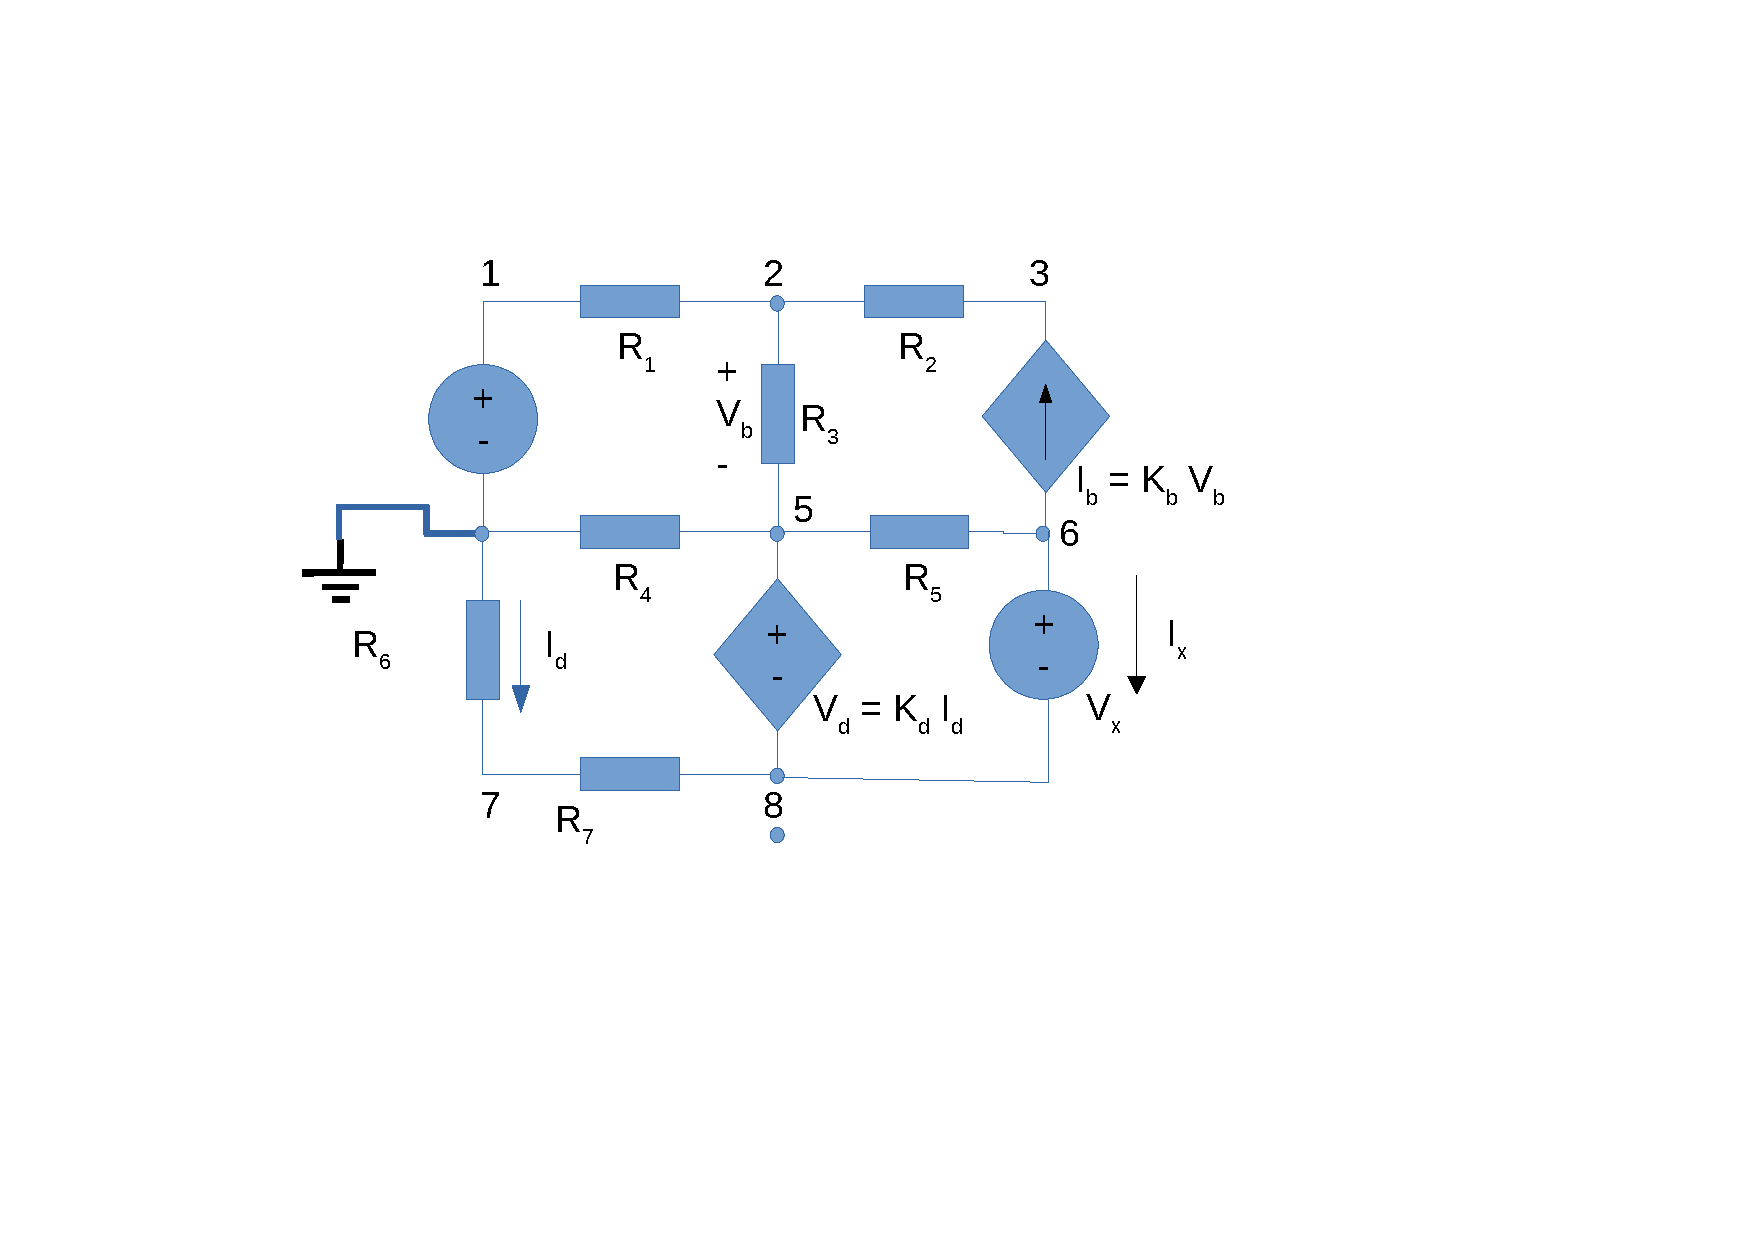
\includegraphics[width=0.8\linewidth]{vx.pdf}
\caption{Circuit for t=0}
\label{fig:zim}
\end{figure}
Now, we only need 6 equations, because the GND node and node 1 become the same node.\\
For node 2, we get:
\begin{equation}
\frac{V_2}{R_1} + \frac{V_2 - V_3}{R_2} + \frac{V_2 - V_5}{R_3} = 0 \Leftrightarrow V_2\left( \frac{1}{R_1} + \frac{1}{R_2} + \frac{1}{R_3} \right) - \frac{V_3}{R_2} - \frac{V_5}{R_3}=0
\end{equation}

For node 3:
\begin{equation}
\frac{V_3 - V_2}{R_2\times K_b }+ V_5 - V_2 = 0 \Leftrightarrow V_2 \left(-\frac{1}{R_2\times K_b} - 1\right) + \frac{V_3}{R_2\times K_b} + V_5 = 0
\end{equation}

For node 5, we get:
\begin{equation} \label{eqn:n5}
  \frac{V_5}{R_4}+ \frac{V_5-V_2}{R_3} + \frac{V_5-V_6}{R_5} + i_d= 0
\end{equation}

Where $i_d$ is the current passing trough the dependent voltage source, $V_d$, ($i_d = -(I_d + I_x)$).

For node 6, we get:
\begin{equation} \label{eqn:n6}
  I_b + \frac{V_6-V_5}{R_5} + I_x = 0 \Leftrightarrow I_x = \frac{V_2-V_3}{R_2} + \frac{V_5-V_6}{R_5}
\end{equation}

And also:
\begin{equation}
V_6-V_8 = V_x
\end{equation}

For node 7:
\begin{equation}
-I_d + \frac{V_7-V_8}{R_7} = 0 \Leftrightarrow \frac{V_7}{R_6} - \frac{V_7-V_8}{R_7} = 0\Leftrightarrow V_7\left(\frac{1}{R_6} + \frac{1}{R_7}\right) - \frac{V_8}{R_7} = 0
\end{equation}

Combining equations (\eqref{eqn:n5}), (\eqref{eqn:n6}) and noticing that $I_d = \frac{V_7-V_8}{R_7}$:
\begin{equation}
V_2 \left( -\frac{1}{R_2} - \frac{1}{R_3}\right) + \frac{V_3}{R_2} +  V_5 \left( \frac{1}{R_3} + \frac{1}{R_4}\right) - \frac{V_7}{R_7} + \frac{V_8}{R_7} = 0
\end{equation}

Knowing that $I_d = \frac{V_d}{K_d}$ and $I_d = \frac{V_7-V_8}{R_7}$, we get the final equation:
\begin{equation}
V_8\left( \frac{1}{R_7} - \frac{1}{K_d}\right) - \frac{V_7}{R_7} + \frac{V_5}{K_d}
\end{equation}


The next step is to solve the following system of equations:
\begin{equation}
\left(\begin{array}{cccccc} \frac{1}{R_1}+\frac{1}{R_2} +\frac{1}{R_3} & -\frac{1}{R_2} & -\frac{1}{R_3} & 0 & 0 & 0\\ -\frac{1}{R_2 K_b}-1 & \frac{1}{R_2 K_b} & 1 & 0 & 0 & 0 \\ -\frac{1}{R_2}-\frac{1}{R_3} & \frac{1}{R_2} & \frac{1}{R_3}+\frac{1}{R_4} & 0& -\frac{1}{R_7} &\frac{1}{R_7} \\ 0&0&0&1&0&-1\\0&0&0&0&\frac{1}{R_6}+\frac{1}{R_7}&-\frac{1}{R_7} \\ 0&0&\frac{1}{K_d}&0&-\frac{1}{R_7}&\frac{1}{R_7}-\frac{1}{K_d}\end{array}\right)
\left(\begin{array}{c} V_2 \\ V_3 \\ V_5 \\ V_6 \\ V_7 \\ V_8 \end{array}\right) 
= \left(\begin{array}{c} 0 \\ 0 \\ 0 \\ V_x \\ 0 \\ 0 \end{array}\right)
\end{equation}

Finally, we can calculate $I_x$ using equation \eqref{eqn:n6}, the equivalent resistance $R_{eq}$ and the time constant, $\tau$: 
\begin{equation}
R_{eq}=\frac{V_x}{I_x}
\end{equation}
\begin{equation}
\tau=R_{eq}\times C
\end{equation}
